% LREC Document Attrition paper, based on ACL2005 example TeX


\documentclass[10pt, a4paper]{article}
% =============================================================================
% Package inclusions
\usepackage{lrec2006}
\usepackage{times}
\usepackage{graphicx}

\usepackage[textsize=tiny]{todonotes}
\usepackage{xcolor}

\usepackage{fancyvrb}

\usepackage[hidelinks]{hyperref}

% =============================================================================
% Custom commands
%\setlength\titlebox{6.5cm}    % Expanding the titlebox

\newcommand{\superscript}[1]{\ensuremath{^{\textrm{#1}}}}
\newcommand{\subscript}[1]{\ensuremath{_{\textrm{#1}}}}
\newcommand{\mon}[1]{{\tt #1}}

% Draft colour
% use \dr{stuff you want redrafting} to highlight something.
\newcommand{\dr}[1]{{\color{blue} #1}}%

% =============================================================================
% Package config
\graphicspath{{./images/}}
\DeclareGraphicsExtensions{.pdf,.png,.jpg}


% =============================================================================
% Title and header content; metadata
% \title{Experiences Scaling an Existing NLP Toolkit: Hansard and USAS}
\title{Experiences with Parallelisation of an Existing NLP Pipeline: Tagging Hansard}


\name{Stephen Wattam\superscript{\small{1}}, Paul Rayson\superscript{\small{1}}, Marc Alexander\superscript{\small{2}} \& Jean Anderson\superscript{\small{2}}}


\address{School of Computing and Communications\superscript{\small{1}} \\
Lancaster University \\
{\tt \{s.wattam, p.rayson\}@lancaster.ac.uk}
\and
	English Language\superscript{\small{2}} \\
University of Glasgow \\
	{\tt \{marc.alexander, jean.anderson\}@glasgow.ac.uk}}

% =============================================================================
\abstract{     This poster describes experiences processing the 2-billion-word Hansard corpus using a fairly standard NLP pipeline on a high performance cluster.  Herein we describe how we were able to parallelise and apply a ``traditional'' single-threaded batch-oriented application to a platform that differs greatly from that for which it was originally designed. We start by discussing the tagging toolchain, its specific requirements and properties, and its performance characteristics.  This is contrasted with a description of the cluster on which it was to run, and specific limitations are discussed such as the overhead of using SAN-based storage. We then go on to discuss the nature of the Hansard corpus, and describe which properties of this corpus in particular prove challenging for use on the system architecture we used. The solution for tagging the corpus is then described, along with performance comparisons against a naive run on commodity hardware.  We discuss the gains and benefits of using high-performance machinery rather than relatively cheap commodity hardware. Our poster provides a valuable scenario for large scale NLP pipelines and lessons learnt from the experience.


% My collided edit:
%
% This poster describes experiences gained in adapting the USAS semantic tagger for use on the Lancaster University high-end computing (HEC) cluster.  We describe the process of tagging the Hansard corpus, comprising 2.2 billion words, by parallelising the existing toolchain: a ``traditional'' single-threaded, batch-oriented system originally designed for execution on low-resource desktop machines.\\
%     We start by discussing the tagging toolchain, its specific requirements and properties, and its performance characteristics.  This is contrasted with a description of the cluster on which it was to run, and specific limitations are discussed, such as the overheads involved in scheduling jobs and accessing SAN-based storage arrays.\\
%     The structure of the Hansard corpus is then described, and it is assessed to identify which aspects prove challenging for use on the cluster.  We describe the solution found, and compare its performance to that of a conventional desktop system in order to evaluate the efficacy of the parallelisation effort.
%     We conclude that many data sets and toolchains may benefit only a little from parallelisation due to the development overhead required, but that this particular data set benefitted greatly from the increased performance high-performance computing hardware affords.
% 



 }

% =============================================================================
% Document body
\begin{document}
\maketitleabstract%

% -------------------------------------------------------------------
\section{Introduction}
\begin{itemize}
    \item What needed doing.
    \item Why this could be interesting to other people.
    \item Other people's use of CLAWS, similar toolchains, HPCs.
    \item Suitability to process massive [big data] corpora with conventional toolkits simply by throwing money/hardware at it.
    \item Signposting.
\end{itemize}


% -------------------------------------------------------------------
\section{Toolchain}
The toolchain being used to tag the corpora was a combination of tools comprising the [?] system.  This consists of a number of smaller tools, each communicating using intermediate files and managed using a series of shell scripts.  We think it's similar to X and Y and has properties transferrable to Z and Z'.



% -------------------------------------------------------------------
\section{High-Performance System}
The system used for processing was the Lancaster university High-End Computing cluster (HEC).  This consists of a number of compute nodes running Scientific Linux\footnote{\url{https://www.scientificlinux.org/}}%
, connected using the Oracle Grid Engine\footnote{\url{http://www.oracle.com/us/products/tools/oracle-grid-engine-075549.html}}.  
In total the system comprises over 2200 CPU cores, 11TB of memory, 32TB of high performance (working) file storage, and a further 1PB of medium performance storage.


\begin{figure}[h]
    \centering
    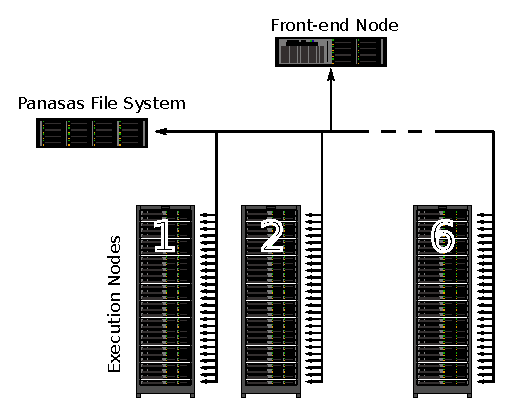
\includegraphics[width=0.5\textwidth]{arch.eps}
    \caption{HEC architecture}
    \label{fig:arch}
\end{figure}

As shown in Figure~\ref{fig:arch}, the system is reliant on network-attached shared storage in the form of a Panasas Activescale Series 8 storage cluster\footnote{\url{http://www.panasas.com/products/activestor-14}}.  Intermediate storage is provided by a number of other storage nodes \todo{Do these provide the working shared storage/scratch, or are they only for use with GridPP?}.

There are 262 compute nodes in total, each with two four- or six-core CPUs\todo{Xeons?} each.  Most of these compute nodes have 24GB of RAM available locally (those that do not have 96GB).

The Oracle Grid Engine scheduling framework works in a batch processing manner, with active jobs competing for access to compute nodes.  This scheduler can be used to queue up job arrays in large batches, which will then be distributed to each compute node individually as they become free.  This was the primary mechanism used to distribute jobs across nodes.




% -------------------------------------------------------------------
\section{The Hansard Corpus}
Hansard is the official published report of both oral and written UK Parliamentary proceedings. It is an edited verbatim report of speeeches in both the House of Commons and the House of Lords. Members' words are recorded by Hansard reporters and then edited to remove repetitions and obvious mistakes but without changing the meaning. Reports of the latest proceedings are published online and updated during the day and can be read online back to 1988\footnote{For more information on Hansard and its history see http://parldisc.jiscinvolve.org/wp/ and http://www.parliament.uk/about/how/publications/hansard/}. 
These records are of importance for scholars of the development of the English language, of British politics and history, and are also used by community-focused organisations.  Historic records back to 1803 have been digitized in XML format and are publically available on the Historic Hansard web site created by the Commons and Lords Libraries and Millbank Systems. There one can search by word or phrase then filter results by speaker or House (Lords or Commons). This is freely available online under an Office of Public Sector Information licence. 
% Together these web sites provide academic and non-academic communities with a significant amount of high-quality data. 
The Hansard corpus is one of the biggest humanities data sets in the UK but was limited in its use by being tagged only by speaker and date. To provide greater utility we wanted the speeches to be searchable by speaker, date, parts of speech (POS) and most interestingly, by topic. This would enhance this significant public material and expose it to new audiences within Higher Education, including linguists, discourse analysts, historians, digital humanists, and cultural scholars. 
We downloaded the XML corpus from the Historic Hansard site, ran routines to standardise the XML coding in order to prepare it for the NLP toolchain. As well as POS tagging, we applied the USAS semantic tagger. Once these annotation steps were complete, we needed to produce word, POS and semantic frequency lists for each speech as per the standard Wmatrix tag wizard pipeline. Finally, in order to expose the key topics of each speech we compared each semantic frequency list to a standard reference corpus, the British National Corpus spoken sampler (one million words) using the log-likelihood statistic to find a set of key semantic tags.

% Glasgow downloaded the XML corpus from the Historic Hansard site, ran routines to standardise the XML coding and then passed the data to Lancaster. UCREL had the knowledge and experience to take on the complex tagging of this very large data set using their established software, the CLAWS part of speech tagger and the USAS semantic tagger.



% \begin{itemize}
%     \item Size
%         \begin{itemize}
%             \item 7545103 XML files in 48,482 directories comprising 2,271,985,142 words and 32.7952GiB of data [inc markup].
%             \item Word sizes: 40, 83, 147, 308, 1400 at 5\%, 25\%, 50\%, 75\% and 95\%.
            % > quantile(words$words, c(.05, .25, .50, .75, .95))
            %   5%  25%  50%  75%  95% 
            %   40   83  147  308 1400
%             \item Average filesize is 2.4KB
%             \item Totals and breakdowns
%         \end{itemize}
%     \item Format
%         \begin{itemize}
%             \item Individual files
%             \item folder structure and organisation (pertinent to later organisation/batching)
%         \end{itemize}
% \end{itemize}

% \subsection{Format}

The full 200-year collection is 2,271,985,142 words and 32.7%952
GiB of data, including mark--up. The corpus is split into 7,545,103 XML files, each representing a speech made in either house of the UK Parliament.  These files are organised into a hierarchical directory structure by house and date, comprising 48,482 folders in total.  A sample of this structure is shown in Figure~\ref{fig:structure}.

\begin{figure}[h]
    \centering
    {
        \small
        \begin{Verbatim}[frame=single]
            Hansard
            +-- Commons
            |   +-- commons 1803-1820
            |   |   \-- commons
            |   |       +-- 1803
            |   |       |   +-- dec
            |   |       |   |   +-- 01
            |   |       |   |   +-- 02
            |   |       |   |   +-- 03
            |   |       |   |   +-- 05
            |   |       |   |   +-- ...
        \end{Verbatim} 
    }
    \caption{Sample directory layout}
    \label{fig:structure}
\end{figure}


\begin{figure}[h]
    \centering
    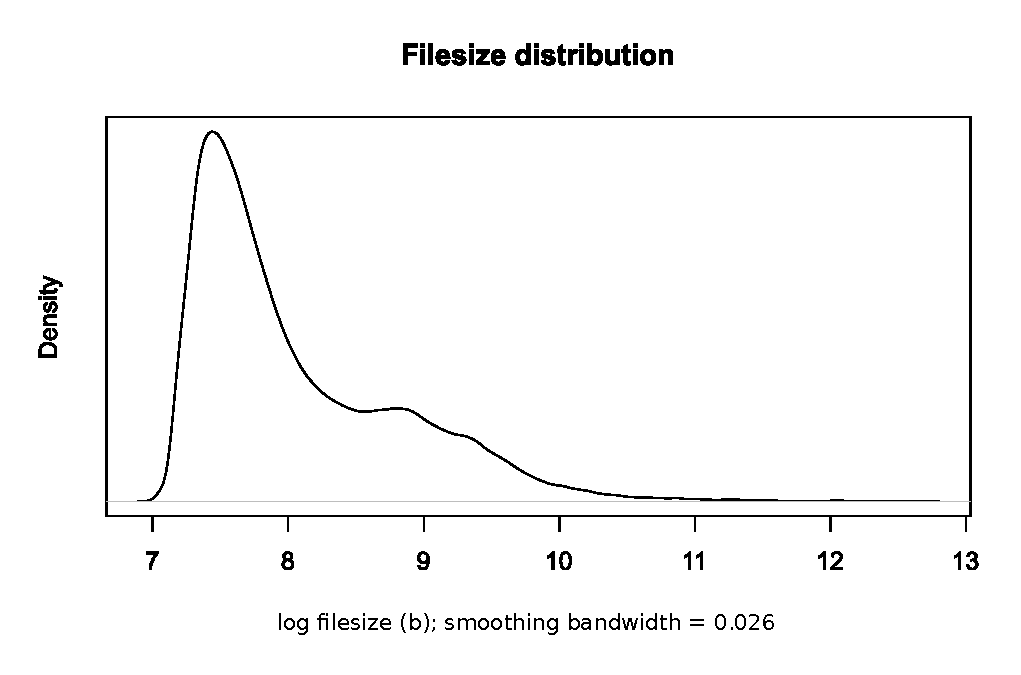
\includegraphics[width=0.5\textwidth]{filesize.eps}


    \begin{tabular}{ | r | c | c | c | c | c | }
        \hline
        Percentile & 5 & 25 & 50 & 75 & 95 \\ \hline
        Words & 40 & 83 & 147 & 308 & 1400 \\ \hline
    \end{tabular}

    \caption{Distribution of log filesizes for all corpus data, and word counts (without markup) for each file.}
    \label{fig:filesizes}
\end{figure}


% \dr{The XML format used contains annotations for X, Y and Z, and follows various conventions...  }

% The XML files themselves follow x format\todo{unsure of this, SW}. 
As shown in Figure~\ref{fig:filesizes}, filesizes are generally small, exhibiting a Zipfian distribution beyond the mode of 1.8KB.  The median size is just 2.4KB, and the 95th percentile is 1.4MB.


% \begin{verbatim}
% > quantile(sizes$filesize, c(.05, .25, .50, .75, .95))
%    5%   25%   50%   75%   95% 
%  1411  1781  2443  5031 14013
% \end{verbatim}


% \subsection{Tagging}
% \begin{itemize}
%     \item What needed tagging
%     \item Which frequencies had to be built (per file/day/totals)
%     \item What work this contributed to
% \end{itemize}



% -------------------------------------------------------------------
\section{Method}
% \subsection{Limitations \& Solutions}

The Wmatrix tag wizard toolchain was originally designed and developed to run on commodity computing hardware in a batch processing fashion.  The toolchain thus respects a number of common limits that apply to desktop computers (e.g. low memory limits) and attempts to exploit other resources that are available in abundance (fast sequential file I/O).
Many of these properties do not transfer to larger clusters, and a number of changes had to be made in order to align the processing stages with the resources available on the HEC system.


\paragraph{File Access}
The Wmatrix toolchain makes extensive use of small output and intermediate files during operation.  This incurs a significant performance overhead when used with filesystems that are typical in high-end distributed systems, which often use large block sizes, carry metadata for versioning and redundancy, or are accessible only over network links.
For this particular process, each input file causes creation of eleven intermediate and output files.  When parallelised, the number of concurrent I/O operations performed, along with the organisation of the corpus (stored as many small files), soon overwhelmed the bandwidth limitations of the shared filesystem.

The solution to this effected changes to the whole toolchain---first, the corpus was restructured to move each day's files into a single \mon{tar} archive.  This could then be copied with a single operation from the shared drive.
This input file was then extracted into a temporary directory on the local disk of the compute node.
Following execution, output was again archived using \mon{tar} and copied back to the shared drive.  This process necessitated a further post--processing stage to extract and validate the output, which was performed after downloading data from the HEC.


\paragraph{Memory Size}
Memory provisions on systems have grown considerably since the toolchain was designed, and as such it fails to exploit even modern desktop systems. The toolchain does this by trading time for space in some instances and by caching data on disk, both of which would have requied significant redevelopment to alter.  We thus elected not to fully exploit each compute node's relatively high 24GB of available memory.




% If we need to further reduce words then this could be thinned out or commented out

\paragraph{Indexing and Co-ordination}
As work was completed away from the shared disk, a system was necessary to co-ordinate compute nodes' access to data.
This was accomplished by using a flatfile, centrally stored and accessed once per batch, that contained a list of input archives and their corresponding output directories.  
The numeric `job ID' environment variable provided by the scheduler was used to compute an offset, which each job used to split the input file by line, selecting a batch of input files for a single job.

The number of input archives tagged per job was chosen to balance scheduling overheads with the need to `smooth out' file access and ensure that any failures did not affect large areas of the corpus.  Ultimately, each job was run using 20 input archives, chosen to take 30 minutes using average input files.



\paragraph{Scheduling Overhead}
The overhead incurred by a shared scheduling system is significant compared to a typical process creation task (exacerbated by the need to copy and extract archives).  This overhead was minimised by tagging multiple directories in a single batch: in practice, running 2230 jobs with a predicted execution time of 30 minutes each, this did not prove to be a limiting factor.
% As mentioned above, scheduling overheads were minimised by tagging multiple directories within a single batch, re-using each compute node many times before copying results back.


\paragraph{Per-node Parallelism}
Each compute node on the HEC is furnished with 8-12 processor cores.  Wmatrix itself does not take advantage of this parallelism, and the decision was made not to introduce the complexity of pipelining into each job dispatch script. 
As such, this remains the largest untapped source of further performance.






% -------------------------------------------------------------------
\section{Performance}
% \begin{itemize}
%     \item When moving processing to a high performance cluster there are two main gains:
%         \begin{itemize}
%             \item Parallelism, which greatly benefits this problem as it is 'embarrassingly parallel'
%             \item Serial speed of each compute node (clusters are usually well specified w.r.t. RAM and CPU provisions)
%         \end{itemize}
% \end{itemize}
% 
% 
% 
% 
% 
% \subsection{HEC}

\begin{figure}[h]
    \centering
    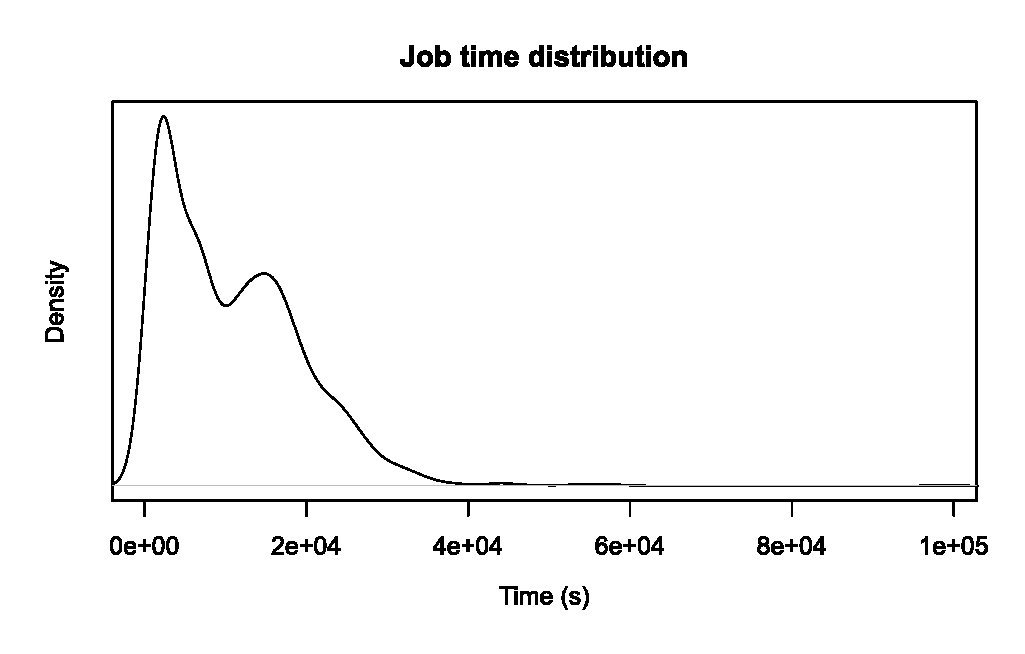
\includegraphics[width=0.5\textwidth]{jobtime.eps}

    \begin{tabular}{ | r | c | c | c | c | c | }
        \hline
        Percentile & 5 & 25 & 50 & 75 & 95 \\ \hline
        Duration & 20m & 53m & 2.5h & 4.5h & 7.3h \\ \hline
    \end{tabular}

    \caption{Distribution of job execution times on the HEC}
    \label{fig:jobtimes}
\end{figure}


% 
% {\small
% \begin{verbatim}
% Total time (s): 24428748    ( / 60 / 60 / 24 = 282 days on the HPC )
% Mean (s): 10955             ( / 60 / 60 = 3.04 hours )
% Min (s): 223                ( / 60 = 3.7 minutes )
% Max (s): 98872              ( / 60 / 60 = 27 hours )
% 
% 
% > quantile(x$time, c(.05, .25, .50, .75, .95))
%        5%       25%       50%       75%       95% 
%  1248.897  3174.155  9321.105 16462.717 26126.913 
%  20 mins   53 mins   2.5 hrs  4.5 hrs   7.25hrs
% \end{verbatim}
% }
% 



The distribution of job durations is shown in Figure~\ref{fig:jobtimes}.  All jobs were complete in 3 days, meaning that the system tagged at a rate of 31.5 million words 
%31,555,349 words 
per hour. Because of the heterogeniety in task length, this rate was not constant, decaying towards the end (the final 231) as the queued tasks ran out and were not replaced.  Had we used larger batches, this effect would have proven more severe as the variance in job length was liable to increase.  Were the corpus particularly large (in the range of hundreds of billions of words), it would be prudent to model and control for this effect ahead of time.
Jobs used a maximum of between 80 and 120MB of memory---our greatest underutilised resource.
% It should be possible to improve the tagging rate by further parallelising within each compute node.  This would theoretically shorten the time spent tagging by a factor of at least 8 to just 9 hours.

% Note that, in order to be evenly divisible by 20, the task list was padded.  This makes the minimum task execution time smaller than it would otherwise be.



\subsection{Commodity Hardware}
In many cases, the alternative to deployment on a HEC cluster will be use of one or many commodity desktop machines.  In order to compare the performance of the toolchain, a random sample of 50 jobs was run through the toolchain using the scheduling scripts described above.

The hardware used was a desktop machine with a single Intel i5 processor, 15GB of memory, and two 7200rpm mechanical hard disks in a RAID-0 configuration.  The system was running Arch Linux\footnote{\url{http://archlinux.org}}, and, as the system is the first author's office machine, work continued on other projects during the benchmarks.  We believe this constitutes a system equivalent to many found across offices today.

\begin{figure}[h]
    \centering
    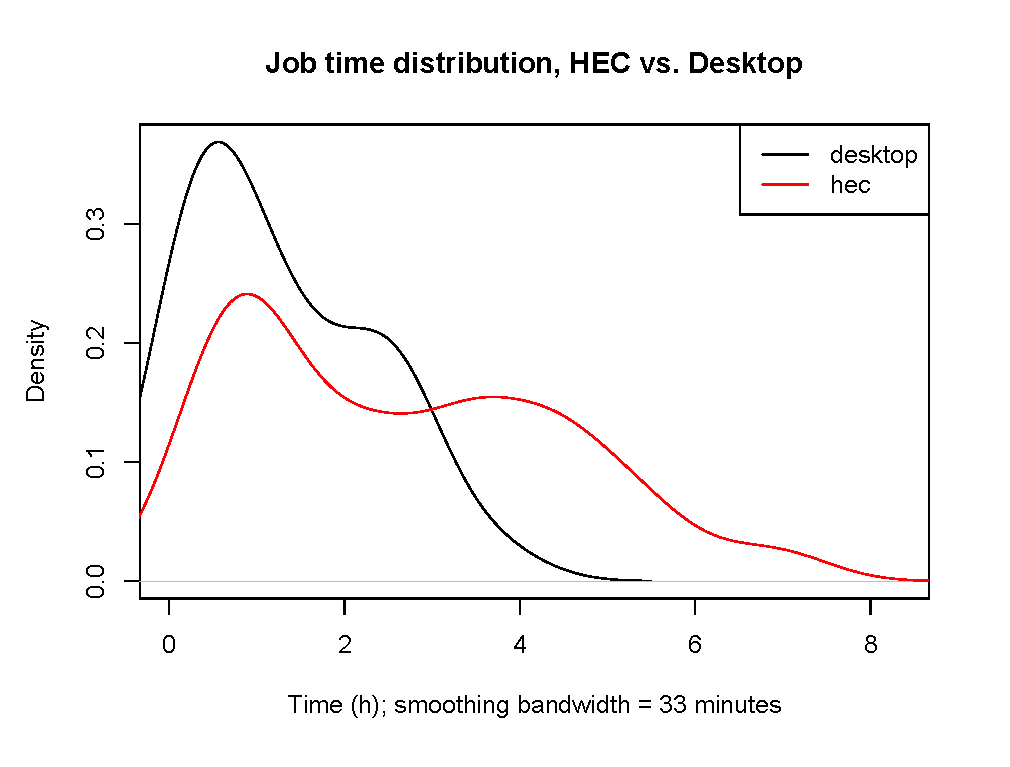
\includegraphics[width=0.5\textwidth]{timecomp.eps}
    % postscript("timecomp.eps", height=5, width=6.5)
    % plot(density(times$tdesk/3600, bw=2000/3600), xlim=c(0, 30000/3600), main="Job time distribution, HEC vs. Desktop", xlab="Time (h); smoothing bandwidth = 33 minutes")
    % lines(density(times$thec/3600, bw=2000/3600), col=2)
    % legend("topright", c("desktop", "hec"), lty=1, col=c(1,2))
    % dev.off();

    % -------------
    % > quantile(times$thec, c(.05, .25, .50, .75, .95))
    %        5%       25%       50%       75%       95% 
    %  1322.534  3404.690  8524.075 14848.393 20306.699 
    % > quantile(times$tdesk, c(.05, .25, .50, .75, .95))
    %         5%        25%        50%        75%        95% 
    %   552.9762  1332.1664  3804.2810  8380.7053 10042.5802 

    \begin{tabular}{ | r | c | c | c | c | c | }
        \hline
        Percentile & 5 & 25 & 50 & 75 & 95 \\ \hline
        HEC        & 22m & 57m & 2.4h & 4.1h & 5.6h \\ \hline
        Desktop    & 9m & 22m & 1h & 2.3h & 2.8h \\ \hline
    \end{tabular}

    \caption{HEC and Desktop job execution times for a sample of 50 jobs}
    \label{fig:timecomp}
\end{figure}


As can be seen in Figure~\ref{fig:timecomp}, the desktop system runs individual jobs significantly faster.  Fitting a linear model indicates that the desktop is able to run jobs approximately 2.1 times faster than a single HEC core.  The same model indicates a 100 second job startup overhead on the HEC (including copying of files).
Had we continued to tag the corpus in this manner, it would have taken 98 days on the desktop system, and thus required at least 33 equivalent machines to achieve the HEC's performance.  It seems unlikely that manually splitting the data across that many systems would save time compared to the development overheads incurred for the HEC tagger.




% -------------------------------------------------------------------
\section{Discussion and conclusion}
% \begin{itemize}
%     \item Compare against the price of manually parallelising on a "few" commodity systems--
%         \begin{itemize}
%             \item Dev time
%             \item Execution time
%             \item Relative speed up
%             \item Relative difficulty avoiding job overheads, etc.
%         \end{itemize}
% \end{itemize}

Two weeks was spent developing and testing the HEC deployment of the toolchain.  Of this, a significant portion was spent adapting the toolchain to run on the scheduler without restriction from the shared filesystem.
The problem is embarrassingly parallel, and the design of many HEC facilities is well suited to exploit that.  It is certainly the case that, even if we had manually split the data and run it on (faster) commodity hardware, we would still have incurred significant overhead in doing so.  Assuming development in that case were simpler and took just a week, we would still require ten desktop systems in order to achieve the same overall completion time.  

It is worth noting that we did not fully exploit the parallel capacity of the cluster, and modifications such as parallelising upon each compute node, or pipelining, would yield vastly improved execution times\footnote{Running once per core would have reduced execution times 8-fold to just 9 hours.}.
Though these incur further development effort, they may be worthwhile for many projects, or be used to extend the lifetime of existing toolchains.

In contrast to manually deploying jobs, where scheduling is automated and fast there is a benefit to having smaller jobs, as they may compete more efficiently for resources (though this must be balanced with the overheads of any scheduling itself).
For problems where time constraints are less severe, the toolchain used is particularly specialised, or the data is less inherently parallel, there may be benefits to the simpler approach.  For our purposes, where the task was extremely parallel, the toolchain easily ported, and the timescale short, the greater concurrency offered by a high performance cluster proved invaluable.  

% --

In future work, we intend to test the HEC facilities with other corpora with different filesize distribution characteristics. We will also experiment with the MapReduce programming model through implementations such as Apache Hadoop. A key future requirement is to expose such parallel processing facilities through a programming-lite interface so that the benefits can be exploited by corpus linguists and digital humanists alike.










% 
% 
% but the HEC incurs severe overheads for some operations that are fast on commodity systems.  This effect is particularly noticable as the toolchain was designed with such systems in mind.  One possible alternative to use of such specialised hardware would be manually parallelising the toolchain over a number of desktop systems.  
% 
% This has a number of advantages in terms of development time, and greatly simplifies the deployment in terms of software requirements (especially as a whole system can then be booted from cloned external disks or the network).  
% 
% 
% In situations where the toolchain to be run is not inherently parallel, and the problem is, this could prove a relative cheap, fast, and easy option.
% 
% \dr{Revise the above when data about relative single-worker speed comes in}
% 
% The structure of the HEC required that jobs were constructed to take a minimum time, in order to minimise the load on I/O systems.  This constraint increases the risk of running wildly heterogenous tasks, something that ultimately reduces the efficiency of the parallelisation as jobs run out.  There are three possible solutions to this: jobs can be made as small as possible whilst testing for I/O stress (this is the approach we used); job duration may be modelled and a batch size chosen to trade off the two properties; or the input data may be re-distributed between to create batches with homogenous runtimes.  The heterogeniety of our runtimes indicates that, for larger corpora where there is are stricter runtime constraints, a mix of these three methods may be necessary to ensure efficient and timely execution.
% 




% =============================================================================
\bibliographystyle{lrec2006}
\bibliography{hansard-lr14}

% =============================================================================
\end{document}

